\documentclass{article}
\usepackage{amsmath}
\usepackage{amssymb}
\usepackage{tikz}
\usepackage{framed}

\title{Mathematical Paper on Algebra 2 Honors}
\author{Badger Code}
\date{\today}

\begin{document}
\maketitle

\section{Polynomials and Rational Expressions}
Polynomials are fundamental algebraic expressions comprised of terms with coefficients and variables raised to non-negative integer powers. A polynomial of degree \(n\) has the general form:
\[ P(x) = a_nx^n + a_{n-1}x^{n-1} + \ldots + a_1x + a_0 \]
where \(a_i\) are coefficients and \(n\) is the highest power.

\begin{framed}
\textbf{Example:}
\[ P(x) = 3x^4 - 2x^2 + 5x + 1 \]
\end{framed}

Rational expressions are ratios of two polynomials, and simplifying them often involves factoring both the numerator and denominator.

\begin{framed}
\textbf{Example:}
\[ R(x) = \frac{2x^2 - 6x}{4x^2 + 8x} = \frac{2x(x - 3)}{4x(x + 2)} = \frac{x - 3}{2(x + 2)} \]
\end{framed}

\section{Complex Numbers}
Complex numbers extend the notion of real numbers by introducing the imaginary unit \(i\), where \(i^2 = -1\). A complex number is represented as \(a + bi\), where \(a\) is the real part and \(b\) is the imaginary part.

\begin{framed}
\textbf{Example:}
\[ z = 3 + 2i \]
\end{framed}

Complex arithmetic includes addition, subtraction, multiplication, and division of complex numbers, following the distributive property.

\begin{framed}
\textbf{Example:}
\[ (2 + 3i) \cdot (1 - 2i) = 8 - i \]
\end{framed}

\section{Quadratic Functions and Equations}
Quadratic functions have the form \(f(x) = ax^2 + bx + c\), and they create parabolic curves. The vertex form of a quadratic function is \(f(x) = a(x - h)^2 + k\), where \((h, k)\) is the vertex.

\begin{framed}
\textbf{Example:}
\[ f(x) = 2x^2 - 4x + 3 \quad \text{has vertex form} \quad f(x) = 2(x - 1)^2 + 1 \]
\end{framed}

Quadratic equations can be solved using the quadratic formula:
\[ x = \frac{-b \pm \sqrt{b^2 - 4ac}}{2a} \]

\begin{framed}
\textbf{Example:}
Solve \(x^2 - 5x + 6 = 0\).
\end{framed}

\begin{tikzpicture}
% Graph of quadratic function
\draw[->] (-1,0) -- (4,0) node[right] {\(x\)};
\draw[->] (0,-1) -- (0,5) node[above] {\(f(x)\)};
\draw[domain=-0.5:3.5,smooth,variable=\x,blue] plot ({\x},{(\x)^2 - 4*\x + 3});
\draw[dashed] (1,0) -- (1,1) node[above] {\((1,1)\)};
\end{tikzpicture}

\section{Exponential and Logarithmic Functions}
Exponential functions have the form \(f(x) = a^x\), where \(a > 0\) and \(a \neq 1\). They exhibit rapid growth or decay.

\begin{framed}
\textbf{Example:}
\(f(x) = 2^x\)
\end{framed}

Logarithmic functions are inverses of exponential functions, defined as \(f(x) = \log_a(x)\).

\begin{framed}
\textbf{Example:}
\(f(x) = \log_2(x)\)
\end{framed}

The properties of logarithms include the product rule, quotient rule, and change of base formula.

\begin{framed}
\textbf{Example:}
Simplify \(\log_3(27) - \log_3(9)\).
\end{framed}

\section{Trigonometry and Circular Functions}
Trigonometry studies the relationships between angles and sides of triangles. Circular functions (sine, cosine, tangent) are essential in trigonometry.

\begin{framed}
\textbf{Example:}
In a right triangle, \(\sin(\theta) = \frac{\text{opposite}}{\text{hypotenuse}}\).
\end{framed}

Trigonometric identities, such as the Pythagorean identities, enable simplification of trigonometric expressions.

\begin{framed}
\textbf{Example:}
Simplify \(\sin^2(\theta) + \cos^2(\theta)\).
\end{framed}

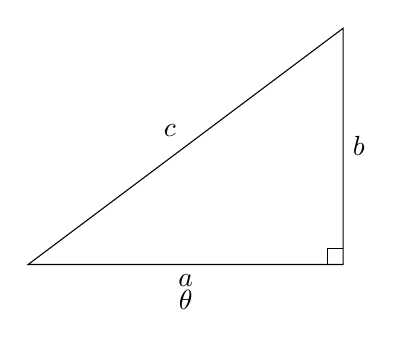
\begin{tikzpicture}
% Right triangle
\draw (0,0) -- (4,0) -- (4,3) -- cycle;
\draw (3.8,0) -- (3.8,0.2) -- (4,0.2);
% Labels
\node[below] at (2,0) {\(a\)};
\node[right] at (4,1.5) {\(b\)};
\node[above left] at (2,1.5) {\(c\)};
\node[below] at (2,-0.2) {\(\theta\)};
\end{tikzpicture}

\section{Matrices and Systems of Equations}
Matrices are arrays of numbers, and matrix operations include addition, subtraction, and multiplication.

\begin{framed}
\textbf{Example:}
\[ A = \begin{bmatrix} 2 & 3 \\ 1 & 4 \end{bmatrix}, \quad B = \begin{bmatrix} -1 & 0 \\ 2 & -3 \end{bmatrix} \]
\end{framed}

Systems of linear equations can be solved using matrix methods like Gaussian elimination.

\begin{framed}
\textbf{Example:}
Solve the system: \(\begin{cases} 2x + 3y = 8 \\ x - 2y = 3 \end{cases}\).
\end{framed}

\section{Sequences and Series}
Sequences are ordered lists of numbers, and series are the sums of these sequences. Arithmetic and geometric sequences are common.

\begin{framed}
\textbf{Example:}
Arithmetic sequence: \(2, 5, 8, 11, \ldots\) \\
Geometric sequence: \(3, 6, 12, 24, \ldots\)
\end{framed}

Infinite geometric series converge if the absolute value of the common ratio is less than 1.

\begin{framed}
\textbf{Example:}
Evaluate \(\sum_{n=1}^{\infty} \frac{1}{2^n}\).
\end{framed}

\section{Polar Coordinates and Parametric Equations}
Polar coordinates describe points in terms of distance (\(r\)) and angle (\(\theta\)).

\begin{framed}
\textbf{Example:}
Point \(P\) in polar coordinates: \((r, \theta)\).
\end{framed}

Parametric equations describe motion using separate equations for \(x\) and \(y\) in terms of a parameter \(t\).

\begin{framed}
\textbf{Example:}
Parametric equations for a circle: \(x = r\cos(t)\), \(y = r\sin(t)\).
\end{framed}

\section{Probability and Statistics}
Probability measures the likelihood of an event occurring. Statistics involves data analysis and interpretation.

\begin{framed}
\textbf{Example:}
Probability of rolling a 6 on a fair die: \(\frac{1}{6}\).
\end{framed}

Expected value is the weighted average outcome of a random variable.

\begin{framed}
\textbf{Example:}
Expected value of rolling a fair die: \(\frac{1}{6}(1) + \frac{1}{6}(2) + \ldots + \frac{1}{6}(6) = 3.5\).
\end{framed}

\section{Conic Sections}
Conic sections result from intersecting a plane with a double-napped cone.

\begin{framed}
\textbf{Example:}
Equation of a circle: \(x^2 + y^2 = r^2\).
\end{framed}

Ellipses, hyperbolas, and parabolas are conic sections with distinct properties.

\begin{framed}
\textbf{Example:}
Equation of a parabola: \(y = ax^2 + bx + c\).
\end{framed}

\section{Functions and Relations}
Functions map each element in the domain to a unique element in the range. Inverses are functions that "reverse" the original function.

\begin{framed}
\textbf{Example:}
Function: \(f(x) = 2x + 1\) \\
Inverse: \(f^{-1}(x) = \frac{x - 1}{2}\)
\end{framed}

One-to-one functions have distinct inputs mapping to distinct outputs.

\begin{framed}
\textbf{Example:}
One-to-one function: \(f(x) = x^3\)
\end{framed}

\section{Advanced Algebraic Techniques}
Polynomial long division and synthetic division aid in polynomial simplification and root finding.

\begin{framed}
\textbf{Example:}
Divide \(3x^3 + 5x^2 - 2x + 1\) by \(x - 2\).
\end{framed}

Partial fraction decomposition is used to break down rational expressions into simpler fractions.

\begin{framed}
\textbf{Example:}
Decompose \(\frac{3x + 4}{x^2 - 5x + 6}\) into partial fractions.
\end{framed}

\section{Analytical Geometry}
Analytical geometry studies the relationship between equations and geometric shapes.

\begin{framed}
\textbf{Example:}
Distance formula between two points \((x_1, y_1)\) and \((x_2, y_2)\): \\
\(d = \sqrt{(x_2 - x_1)^2 + (y_2 - y_1)^2}\)
\end{framed}

Midpoint formula finds the midpoint between two points.

\begin{framed}
\textbf{Example:}
Midpoint between \((x_1, y_1)\) and \((x_2, y_2)\): \\
\(\left(\frac{x_1 + x_2}{2}, \frac{y_1 + y_2}{2}\right)\)
\end{framed}

\section{Conclusion}
Algebra 2 Honors explores a rich array of mathematical concepts that deepen your understanding of algebra, trigonometry, and analytical geometry. These concepts provide a foundation for advanced studies and applications in various fields. Through this paper, we've delved into polynomial operations, complex numbers, quadratic functions, exponential functions, trigonometric identities, matrix operations, sequences and series, and much more. The intricate interplay of these concepts equips you with a powerful toolkit for problem-solving and mathematical exploration.

\end{document}